\documentclass[anon]{CI}
\usepackage[latin1]{inputenc}
\usepackage[english]{babel}

% The following packages will be automatically loaded:
% amsmath, amssymb, natbib, graphicx, url, algorithm2e

\title[CI Project]{Swarm intelligence for counting the degrees of separation in Twitter}

 % Use \Name{Author Name} to specify the name.
 % If the surname contains spaces, enclose the surname
 % in braces, e.g. \Name{John {Smith Jones}} similarly
 % if the name has a "von" part, e.g \Name{Jane {de Winter}}.
 % If the first letter in the forenames is a diacritic
 % enclose the diacritic in braces, e.g. \Name{{\'E}louise Smith}

 % Two authors with the same address
  % \coltauthor{\Name{Author Name1} \Email{abc@sample.com}\and
  %  \Name{Author Name2} \Email{xyz@sample.com}\\
  %  \addr Address}

 % Three or more authors with the same address:
 % \coltauthor{\Name{Author Name1} \Email{an1@sample.com}\\
 %  \Name{Author Name2} \Email{an2@sample.com}\\
 %  \Name{Author Name3} \Email{an3@sample.com}\\
 %  \addr Address}


 % Authors with different addresses:
 \author{\Name{�lex Pardo Fernandez} \Email{alexpardo.5@gmail.com}\\
 \AND
 \Name{David S�nchez Pinsach} \Email{sdividis@gmail.com}\\
 }

\begin{document}

\maketitle

\begin{abstract}
This is a great project and therefore it has a concise abstract.
\end{abstract}

\begin{keywords}
Swarm Intelligence, Ant Colony Optimization, Twitter, Degrees of Separation.
\end{keywords}


\section{Problem statement and goals}

%\textbf{This is where the content of your paper starts. Remember:
%\begin{itemize}
%\item Limit the main text (without bibliography and appendices) to 10 pages.
%\item Include, either in the main text or the appendices, enough details to convince the lecturers of the project's merits.
%\item You should cite all relevant references, including your own.
%\end{itemize}}
A characteristic of the humans are the sociability and that means how to communicate with each others or how the humans are connected in order to share information, knowledge, tasks and so on. In this line, exists some theories about the sociability which try to focus on some characteristics about these relationships between humans.
\\\\
On the one hand, the theory of the six degrees was originally set out by \emph{Frigyes Karinthy} and explains that everyone is connected to any other person in the world by six degrees. That means, if you want to know or to arrive a message to someone in the world, you will need to pass by other four persons, as maximum, between you and your objective. During these last decades, the six degree theory has been used in many fields like economy, social networks, markets and so on and the concept is focused on the connectivity between things like humans, markets or node and it is usual applied in a networks.
\\\\
On the other hand, Twitter is the one of the most social networks that has grown quickly these last years. The main idea is to create a shorts messages of the 140 characters in order to communicate your ideas or your opinions in a quickly way. Moreover, Twitter have made some concepts that are very popular now as are the \emph{trending topic}, \emph{tweet}, \emph{followers}, \emph{followings} or \emph{hash-tag}.
\\\\
The main objective of this work will be estimate the degrees of separation in Twitter and it is possible to obtain six degrees of separation between two random people. In order to do this task, it will use some ideas of the Computational Intelligence like Swarm Intelligence with Ant Colony Optimization(AC0) technique.

%Content:
%\begin{enumerate}
%\item Explain theory of the 6 degrees
%\item Define the network
%\item Goals: estimate the degrees of separation in twitter
%\end{enumerate}


\newpage

\section{Previous work}

The previous work is based on these ideas:
\begin{itemize}
\item ACO original \citep{Colorni91}: Explain the algorithm of the Ant Colony Optimization.
\item General theory \citep{watts}: Explain the general theory about the six degree.
\item On Twitter as \citep{cheng}: Explain the six degree on the Twitter network.
\item On other social nets such as


\end{itemize}

\section{The CI methods}

Swarm intelligence is a natural method based in the behaviour of the decentralized individuals who obtain solutions in some problem as result of their interactions. These agents normally are simple, with a few capabilities and follow simple rules. It includes ant colony optimization, flocking of the birds, bacterial grow or some on. 
\\\\
As it mention previously, it will use the Ant Colony Optimization algorithm in order to obtain the degree of separation of two random person. In this type of algorithm the individuals are the ants who have few capabilities. The ants cannot communicate with the others and only use the trace of pheromone as a probabilistic method in order to obtain the choice when they have different options. When a ant travels although the two points it leaves a few of pheromone. The other ants around these points feel the pheromone and try to follow this path. The paths with few pheromone will have less probability than the path with high pheromone. As shows the figure \ref{fig:aco}, the ants converges to the shortest path between two points and this is the main characteristic of this method. We will use this idea of the shortest path between two points, as a minimum degree between two person in the Twitter network environment. In the appendix \ref{implementation}, it will show how the algorithm works in details.

\begin{figure}[htb!]
\centering
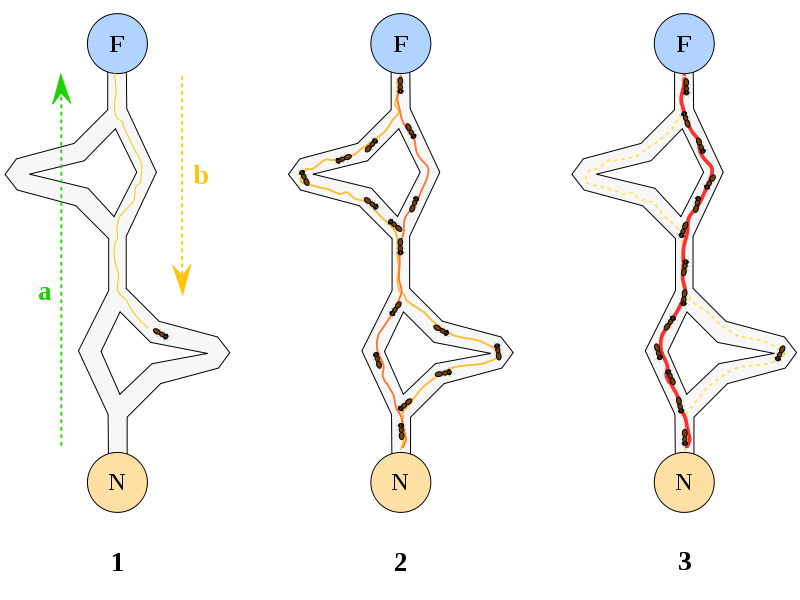
\includegraphics[width=0.6\textwidth]{img/aco}
\caption{ACO algorithm}
\label{fig:aco}
\end{figure}

\section{Results and Discussion}

\section{Extensions, strengths and weaknesses}

\section{Conclusions}

\bibliography{bibliography.bib}

\appendix


\section{Implementation details} %(if applicable)
\label{implementation}

The application have been coded with the Python 2.7 language version. It consists in a script which contains a main function with other internal function in order to give us the result of the execution.

We based the code in the next basic pseudo-code algorithm of the ACO:
\\
�put here pseudocode!
\\
Next to the pseudo-code we want to enter a few detail of some parts of the code and how this parts had been coded.
\begin{itemize}
\item \textbf{Pheromone}: The pheromone is the most important part of the our problem and our code. Remember that the ants try to follow the path which contain high quantity of pheromone. However the pheromone effect disappears with the time. For this reason, the algorithm need to define two parameters in order to determine the quantity of the pheromone that leaves the ant and the quantity of the pheromone disappears at each turn.

\item \textbf{Start and final points of the ants}: We select always randomly the start and the final point of the ants using the standard Random methods of the python.
\end{itemize}

\end{document}
